\documentclass[a4paper]{article}

% Pacotes para o português.
\usepackage[brazilian]{babel}
\usepackage[utf8]{inputenc}
\usepackage[T1]{fontenc}

\usepackage{datetime}
\usepackage{graphicx}

% Usado nos pedaços de código.
\usepackage{listings}
\lstset{language=C,
	basicstyle=\small\sffamily,
	numbers=left,
	numberstyle=\tiny,
	frame=tb,
	columns=fullflexible,
	showstringspaces=false,
	captionpos=b}
\renewcommand\lstlistingname{Código}

\newcommand{\HRule}{\rule{\linewidth}{0.5mm}}

\begin{document}

\begin{titlepage}
\begin{center}	

% Topo 1.
\textsc{\Large UNIVERSIDADE DE SÃO PAULO\\
	INSTITUTO DE CIÊNCIAS MATEMÁTICAS E DE COMPUTAÇÃO}\\[0.7cm]

% Topo 2.
\textsc{\Large SSC0143}\\[0.2cm]
\textsc{\Large Programação Concorrente - Turma B}\\[0.5cm]

% Título.
\HRule \\[0.4cm]
{ \huge \bfseries Jacobi-Richardson}\\[0.4cm]
\HRule \\[0.4cm]
\textsc{Professor Dr. Julio Estrella}\\[1.5cm]

% Grupo
\begin{minipage}{0.4\textwidth}
\begin{flushleft} \large
\emph{Grupo 06:}\\
Bruno Junqueira Adami\\
Lucas Junqueira Adami\\
Lucas Lobosque\\
\end{flushleft}
\end{minipage}
\begin{minipage}{0.4\textwidth}
\begin{flushright} \large
\emph{Números USP:}\\
6878762\\
6792496\\
6792645\\
\end{flushright}
\end{minipage}

\vfill

% Rodapé.
{\large \today}
	
\end{center}
\end{titlepage}

\section{Introdução}
\indent \indent Sistemas lineares são descritos conforme a Equação~\ref{eq-axb}. A matriz \emph{A} do sistema linear pode ser decomposta na forma descrita pela Equação~\ref{eq-aldr} e ser reduzida conforme a Equação~\ref{eq-alir}.
\begin{eqnarray} \label{eq-axb}
	Ax = b
\end{eqnarray}
\begin{eqnarray} \label{eq-aldr}
	A = L + D + R
\end{eqnarray}
\begin{eqnarray} \label{eq-alir}
	A^\star = L^\star + I + R^\star 
\end{eqnarray}
\indent Usando essas decomposições, é possível apresentar o processo iterativo chamado de método de Jacobi-Richardson definido na Equação~\ref{eq-jr}. O processo de parada do método é definido na Equação~\ref{eq-stp}. Para garantir a convergência, a matriz \emph{A} deve ser estritamente diagonalmente dominante, satisfazendo o critério das linhas e colunas.
\begin{eqnarray} \label{eq-jr}
	x^{(k+1)} = -(L^\star + R^\star)x^{(k)} + b^\star
\end{eqnarray}
\begin{eqnarray} \label{eq-stp}
	\frac{\parallel x^{(k)} - x^{(k-1)}\parallel_\infty}{\parallel x^{(k)}\parallel_\infty} < \epsilon
\end{eqnarray}
\indent Apresentado os conceitos necessários, o objetivo do trabalho é a implementação do método de Jacobi-Richardson utilizando uma abordagem sequencial e uma paralela usando OpenMP e MPI. Ao final, há uma discução dos resultados obtidos pelas duas abordagens.

\section{A abordagem sequencial}
\indent \indent A abordagem sequencial do método não tem segredos. Ela segue os passos do algoritmo fielmente. Primeiro, o programa carrega o arquivo de entrada. Logo após, ele aplica o método de Jacobi-Richardson. No final, o resultado da execução é mostrada de acordo com a especificação do trabalho.

\section{A abordagem paralela}
\indent \indent A abordagem paralela segue a linha do programa sequencial decompondo-o em partes paralelas. O método pode ser considerado como um algoritmo iterativo paralelo. Isto é, a cada iteração, cada \begin{math}x^{(k)}_i\end{math} pode ser calculado independentemente das outras variáveis na mesma iteração. Portanto, é possível aplicar uma decomposição de dados, onde a cada passo, o vetor \emph{x} é distribuído entre os nós para ser calculado, cada nó recebendo uma faixa de variáveis, conforme ilustra a Figura~\ref{pic-dec}.\\
\begin{figure}[float=h!]
	\centerline{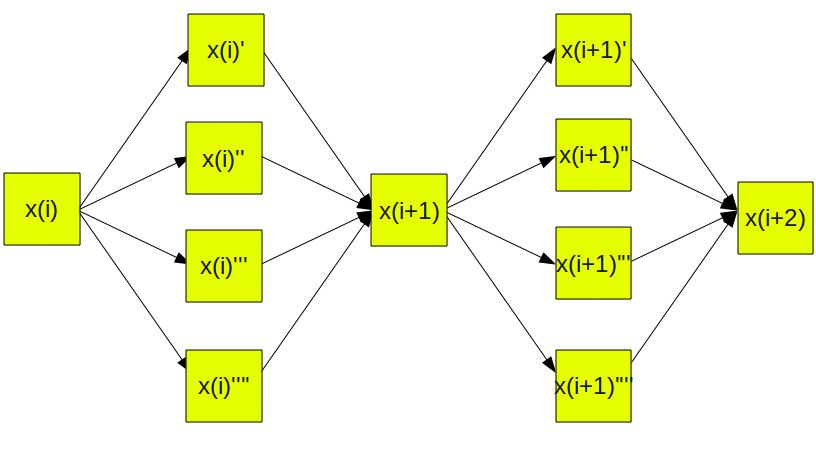
\includegraphics[width=285px, height=161px]{dec}}
	\caption{Decomposição de dados}
	\label{pic-dec}
\end{figure}
\indent O fluxo de dados segue a lógica da Figura~\ref{pic-data}. O primeiro processo, o processo mestre é responsável pela administração de toda a execução. Ele carrega os arquivos de entrada, controla a cadeia de mensagens, envia aos outros processos pedaços do problema e verifica a condição de parada.\\
\indent Em relação à matriz \emph{A}, o processo principal contém todos os seus valores, obtidos durante o carregamento do problema. Quanto aos processos secundários, o mestre envia a eles somente a faixa necessária para que eles possam executar o processo. Isto é feito através da chamada \emph{scatter} do MPI. Essa abordagem é possível pelo fato de que para o cálculo de \begin{math}x_i\end{math}, somente a linha \emph{i} da matriz \emph{A} é necessária.\\
\indent O mesmo ocorre com o vetor \emph{b}. Para calcular \begin{math}x_i\end{math}, somente o valor da posição \emph{i} do vetor \emph{b} é necessário. Uma chamada à função \emph{scatter} é feita e cada processo secundário somente trabalha com a faixa que lhe diz respeito.\\
\indent Para o vetor \emph{X}, é necessário a cada iteração ter todo o seu conteúdo completo. Portanto, um \emph{broadcast} do MPI é feito pelo processo mestre a todos os processos antes que as iterações comecem (\begin{math}x^{(0)}\end{math}).\\
\indent Ao término de cada iteração, os valores obtidos estão armazenados no vetor \emph{X\_}, cada processo contendo sua faixa de valores. Para prosseguir com a próxima iteração, o \emph{allgather} do MPI é chamado sobre o vetor \emph{X}, garantindo a atualização desse vetor a todos os nós.\\
\begin{figure}[float=h!]
	\centerline{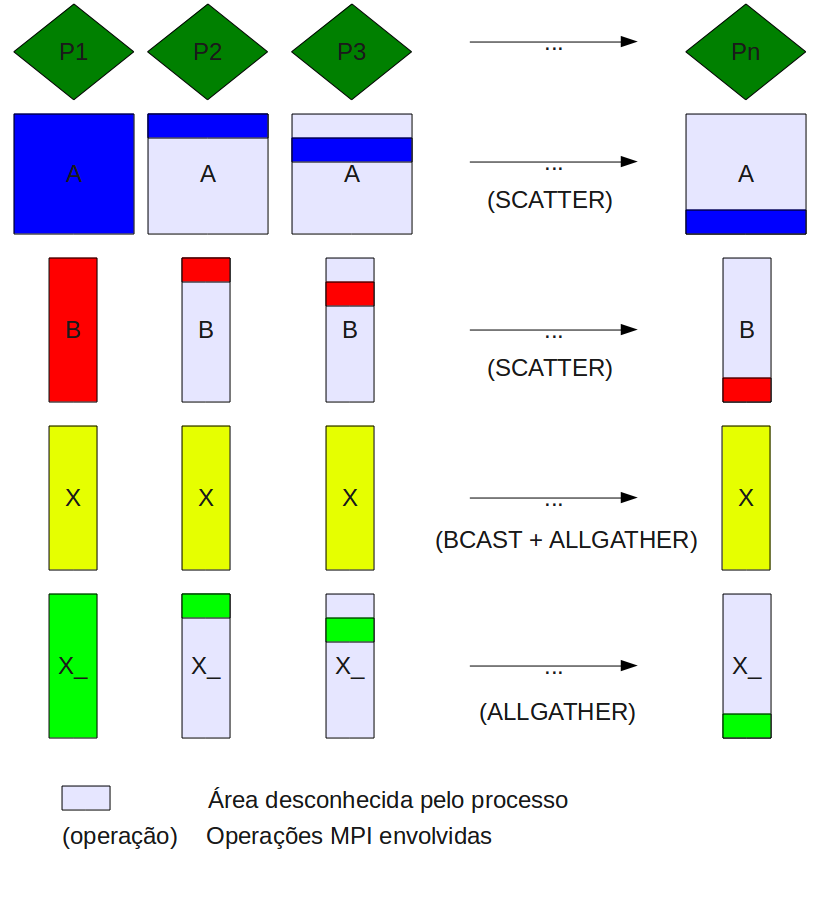
\includegraphics[width=285px, height=315px]{data}}
	\caption{Fluxo de dados}
	\label{pic-data}
\end{figure}
\indent Os macros OpenMP foram utilizados com 4 threads. Há um macro para paralelizar o processo de normalização da matriz \emph{A} antes do início do algoritmo. Há também um macro que paraleliza o cálculo de todos os \begin{math}x_i\end{math} pertencentes à faixa do processo. Para cada \begin{math}x_i\end{math}, outro macro é utilizado na multiplicação feita entre o vetor \emph{x} e a linha \emph{i} da matriz \emph{A}. Um macro foi criado para checar a condição de parada do algoritmo (definido na Equação~\ref{eq-stp}). Finalmente, um último macro é usado para obter a solução do problema.

\newpage
\section{Resultados e conclusões}
\indent \indent Os experimentos consistem em 3 tipos de execução: sequencial, paralela com 5 nós e paralela com 10 nós. Cada configuração foi executada 7 vezes, seguindo uma ordem circular. As médias dos tempos de execução foram tiradas a partir dos resultados e a Tabela~\ref{tab-speedups} mostra os speed-ups dos programas.\\
\indent Segundo a tabela, o programa sequencial é melhor para matrizes pequenas, de tamanho até 500. Para a execução de 5 nós, o speed-up só foi bom quando esse tamanho chega a 1500. Já para 10 nós, é possível perceber que na matriz de tamanho 500, há uma competição entre os programas paralelo e sequencial. Para as matrizes maiores que esse tamanho, essa configuração obteve tempos muito bons.\\
\begin{table}[float=h!]\footnotesize \centerline{\begin{tabular}{|l|l|l|}
	\hline
	Tamanho da matriz 	& Paralelo c/ 5 nós 	& Paralelo c/ 10 nós 	\\ \hline
	250 			& 38\%			& 33\%			\\ \hline
	500 			& 75\% 			& 97\%			\\ \hline
	1000 			& 57\% 			& 142\%			\\ \hline
	1500 			& 117\% 		& 201\%			\\ \hline
\end{tabular}} \caption{Speed-ups} \label{tab-speedups} \end{table}

\indent A Figura~\ref{pic-graph} ilustra os tempos para o algoritmo resolver os problemas dos 3 tipos de execução. O eixo x representa o tamanho da matriz enquanto o eixo y diz respeito ao tempo de execução em segundos. Olhando para o gráfico, conclui-se que com o aumento das matrizes, a execução paralela é melhor que a sequencial, com a configuração de 10 nós sendo melhor que a de 5 nós.\\
\begin{figure}[float=h!]
	\centerline{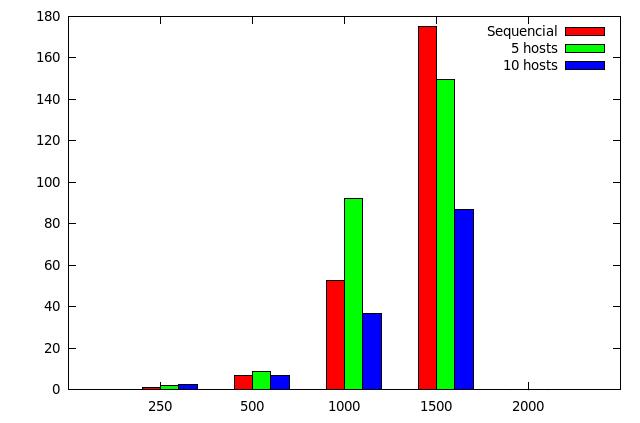
\includegraphics[width=344px, height=227px]{graph}}
	\caption{Gráfico de tempos}
	\label{pic-graph}
\end{figure}

\indent O fato de que para matrizes pequenas o programa sequencial é melhor que o paralelo pode ser explicado através da Equação~\ref{eq-tmp}. Isto é, o tempo que o algoritmo sequencial leva para calcular todo o vetor \emph{x} é menor que o tempo que cada nó \emph{j} leva para calcular sua faixa de \emph{x} (começando em \emph{\begin{math}a_j\end{math}} e terminando em \emph{\begin{math}b_j\end{math}}) mais o tempo gasto na propagação dos resultados dos nós.
\begin{eqnarray} \label{eq-tmp}
	t(x) \le t(\sum_{i=a_j}^{b_j}x_i) + t(propagacao) \qquad \textrm{todo j}
\end{eqnarray}

\begin{thebibliography}{99}
	\bibitem[Jacobi-Richardson]{jari} Franco, Neide Bertoldi; Cálculo Numérico - São Paulo: Pearson Prentice Hall, 2006
	\bibitem[OpenMP]{mp1} http://bisqwit.iki.fi/story/howto/openmp/
	\bibitem[OpenMP]{mp2} http://openmp.org/wp/
	\bibitem[MPI]{mpi1} http://www.slac.stanford.edu/comp/unix/farm/mpi.html
	\bibitem[MPI]{mpi2} http://www.eecis.udel.edu/\~{}saunders/courses/372/01f/manual/manual.html
\end{thebibliography}
\end{document}
